\documentclass[11pt]{article}
\usepackage[a4paper,margin=2cm]{geometry}
\usepackage[brazilian]{babel}
\usepackage[utf8]{inputenc}
\usepackage[T1]{fontenc}
\linespread{1.3}
\parskip=12pt
\parindent=0pt
\usepackage{enumitem}
\usepackage{amsmath}
\usepackage{amsfonts}
\usepackage{graphicx}
\usepackage{amssymb}
\usepackage{hyperref}
\usepackage{amsthm}
\usepackage{color}
\usepackage{placeins}


% Defining the question styles
\theoremstyle{definition}
\newtheorem{prob}{Problema}

% Custom commands
\newcommand{\E}{\mathbb{E}}
\newcommand{\Var}{\mathrm{Var}}
\newcommand{\Prob}{\mathbb{P}}

% declare a new theorem style
\newtheoremstyle{solution}%
{1pt}% Space above
{1pt}% Space below 
{\itshape\color{red}}% Body font
{}% Indent amount
{\bfseries\color{red}}% Theorem head font
{.}% Punctuation after theorem head
{.5em}% Space after theorem head
{}% Theorem head spec (can be left empty, meaning ‘normal’)

\theoremstyle{solution}
\newtheorem*{solution}{Solution}

% --- Code starts here ---
\begin{document}
	\begin{center}
		{\Large{\textbf{Lista III - Métodos Numéricos}}}\\
		\vspace{0.2cm}
		EPGE - 2018\\
		Professor: Cézar Santos\\
		Aluno: Raul Guarini Riva
	\end{center}
	
\begin{prob}
	Segui a mesma calibração da lista anterior e encontrei as funções política do consumo e do capital através da técnica de colocação aliada aos polinômios de Chebyshev. O código principal da lista está no arquivo \texttt{ps3.m}. O tempo de execução desta técnica de projeção espectral foi o menor dentre todas as técnicas até agora (desde a Lista 2): ao redor de 0.4 segundos.
	
	A discretização do processo estocástico da TFP foi feito através da técnica de Tauchen, da mesma maneira das outras listas. Utilizei 7 polinômios de Chebyshev para computar a projeção ($d = 6$, na notação dos slides). O problema é muito bem comportado e, portanto, não foi necessário $d$ muito grande. Testei dimensões maiores mas os valores correspondente de $\gamma_{j}$ rapidamente iam para zero, indicado não ser necessário mais graus de liberdade para a projeção.
	
	A função \texttt{chebyshev\_poly} computa raízes de um polinômio de Chebyshev de ordem $k$ e pode avaliá-lo em qualquer ponto de $[-1,1]$. A função \texttt{C\_proj} computa a projeção da função política do consumo dado um vetor $(d+1)$-dimensional $\gamma$ e um grid no qual o valor do capital de interesse se encontra. Finalmente a função \texttt{risk\_function} computa o resíduo\footnote{Não sei bem o motivo, mas de alguma forma achei que o $R(\gamma, K)$ dos slides era ``Risk'' e não ``Residual''. Implementei tudo e usei a função várias vezes, só notei no final a confusão. Achei que iria semear bugs se trocasse o nome, então deixei desse jeito. Desculpa!} da projeção. É esta a função que define o sistema de $(d+1)$ equações que a função do MATLAB \texttt{fsolve} resolve. A próxima figura ilustra as funções política e Euler Errors.
	\begin{figure}[ht!]
		\centering
		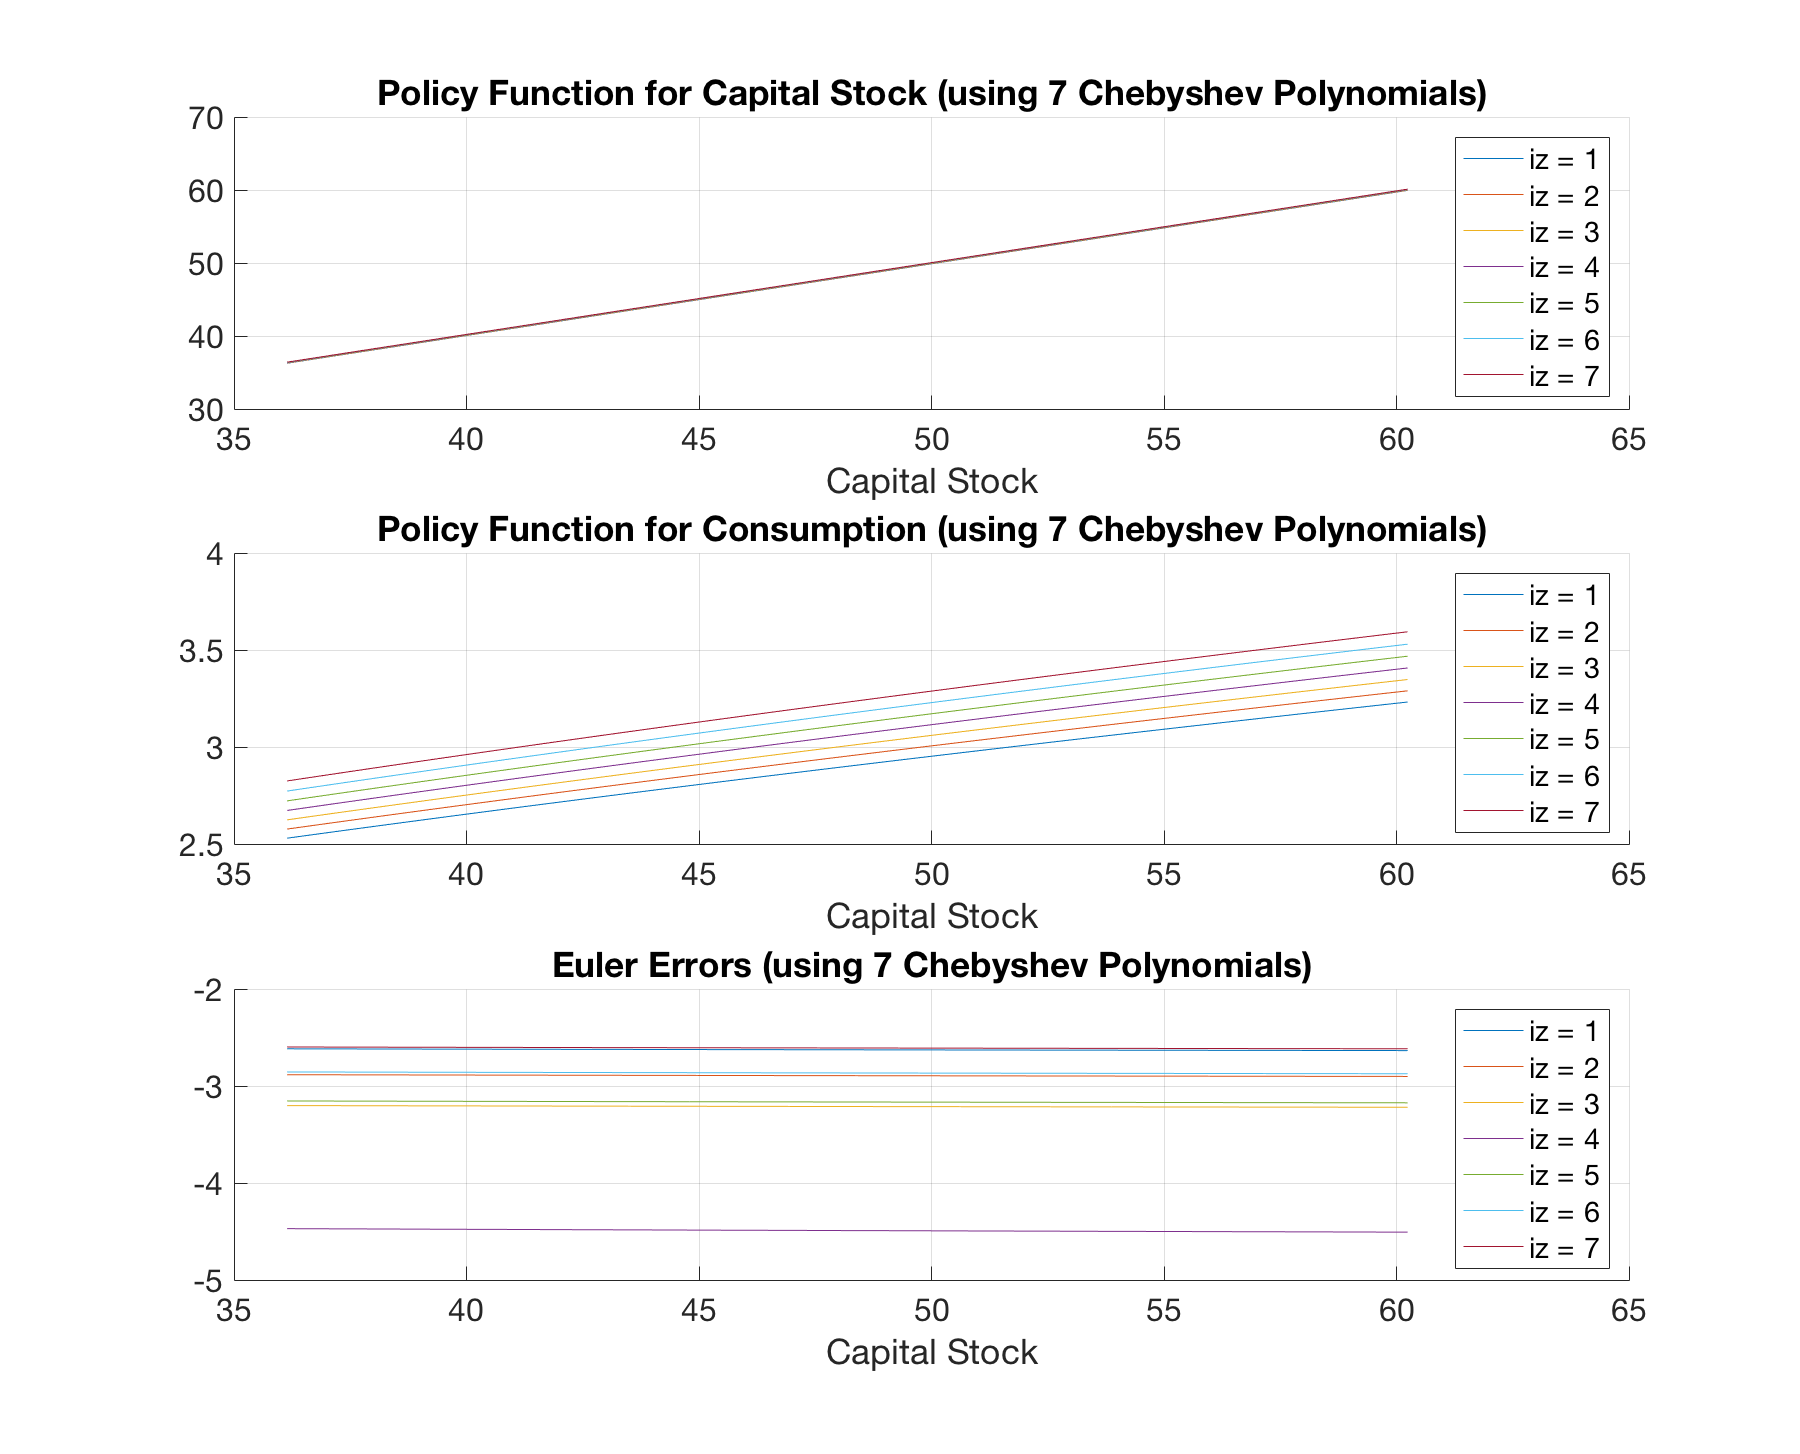
\includegraphics[scale=0.25]{item1.png}
	\end{figure}
	
	Assim como antes, a função política do capital é praticamente linear e não varia muito de acordo com a TFP. Entretanto, níveis maiores de TFP levam a níveis maiores de capital no próximo período, dado o mesmo capital inicial. Este tipo de monotonicidade também é verificada na função política do consumo. Nota-se que esta tem maior curvatura do que a função política do capital.
	
	Curiosamente, o aspecto das curvas de Euler Errors é diferente daquele encontrado, por exemplo, na implementação do grid endógeno na Lista 2. As curvas do erro são basicamente funções constantes de $k$ mas apresentam um comportamento interessante em $z$. Prestando atenção na legenda, vemos que o menor erro de aproximação foi alcançado no valor central do grid de $iz = 4$ e as outras curvas parecem estar dispostas duas a duas de acordo com a distância ao centro. Quanto mais próximo a este, menor o erro de aproximação. Apesar desta observação, não consegui interpretar este resultado.
\end{prob}

\FloatBarrier
\begin{prob}
	Resolvi primeiro o problema utilizando o método da colocação e elementos finitos. Esta abordagem se mostrou também bastante rápida comparada aos métodos da Lista 2, ainda que tenha tido desempenho ligeiramente pior do que a solução usando Polinômios de Chebyshev: 0.62 segundos.
	
	Dividi o intervalo correspondente ao grid do capital (o mesmo das outras questões) em 50 elementos finitos, isto é, 50 subintervalos. Dentro de cada elemento, fitei uma função afim do capital do tipo $\text{intercepto}_{i} + a_{i}k$, quando o valor $k$ cai no $i$-ésimo elemento. Portanto, computei ao todo 100 parâmetros. Para tal, utilizei o método da colocação em 100 pontos linearmente espaçados ao longo do grid original do capital.
	
	A função \texttt{find\_element} indica em qual elemento determinado valor de $k$ se encontra utilizando o método ``Divide and Conquer'' dos slides, visando aumentar a performance nesta parte do algoritmo. A função \texttt{C\_proj\_finel} é análoga à função \texttt{C\_proj} e computa, dados os parâmetros, um valor de $z$ e um valor de $k$, o consumo ótimo. Por último, a função \texttt{risk\_function\_finel} computa\footnote{O mesmo disclaimer sobre Risk e Residual...} o vetor de resíduos que a rotina \texttt{fsolve} tentará igualar a zero tendo os 100 parâmetros em questão como graus de liberdade.
	
	A próxima figura ilustra a função política do capital induzida pela função política do consumo, a própria função política do consumo e os Euler Errors:
	\begin{figure}[h!]
		\centering
		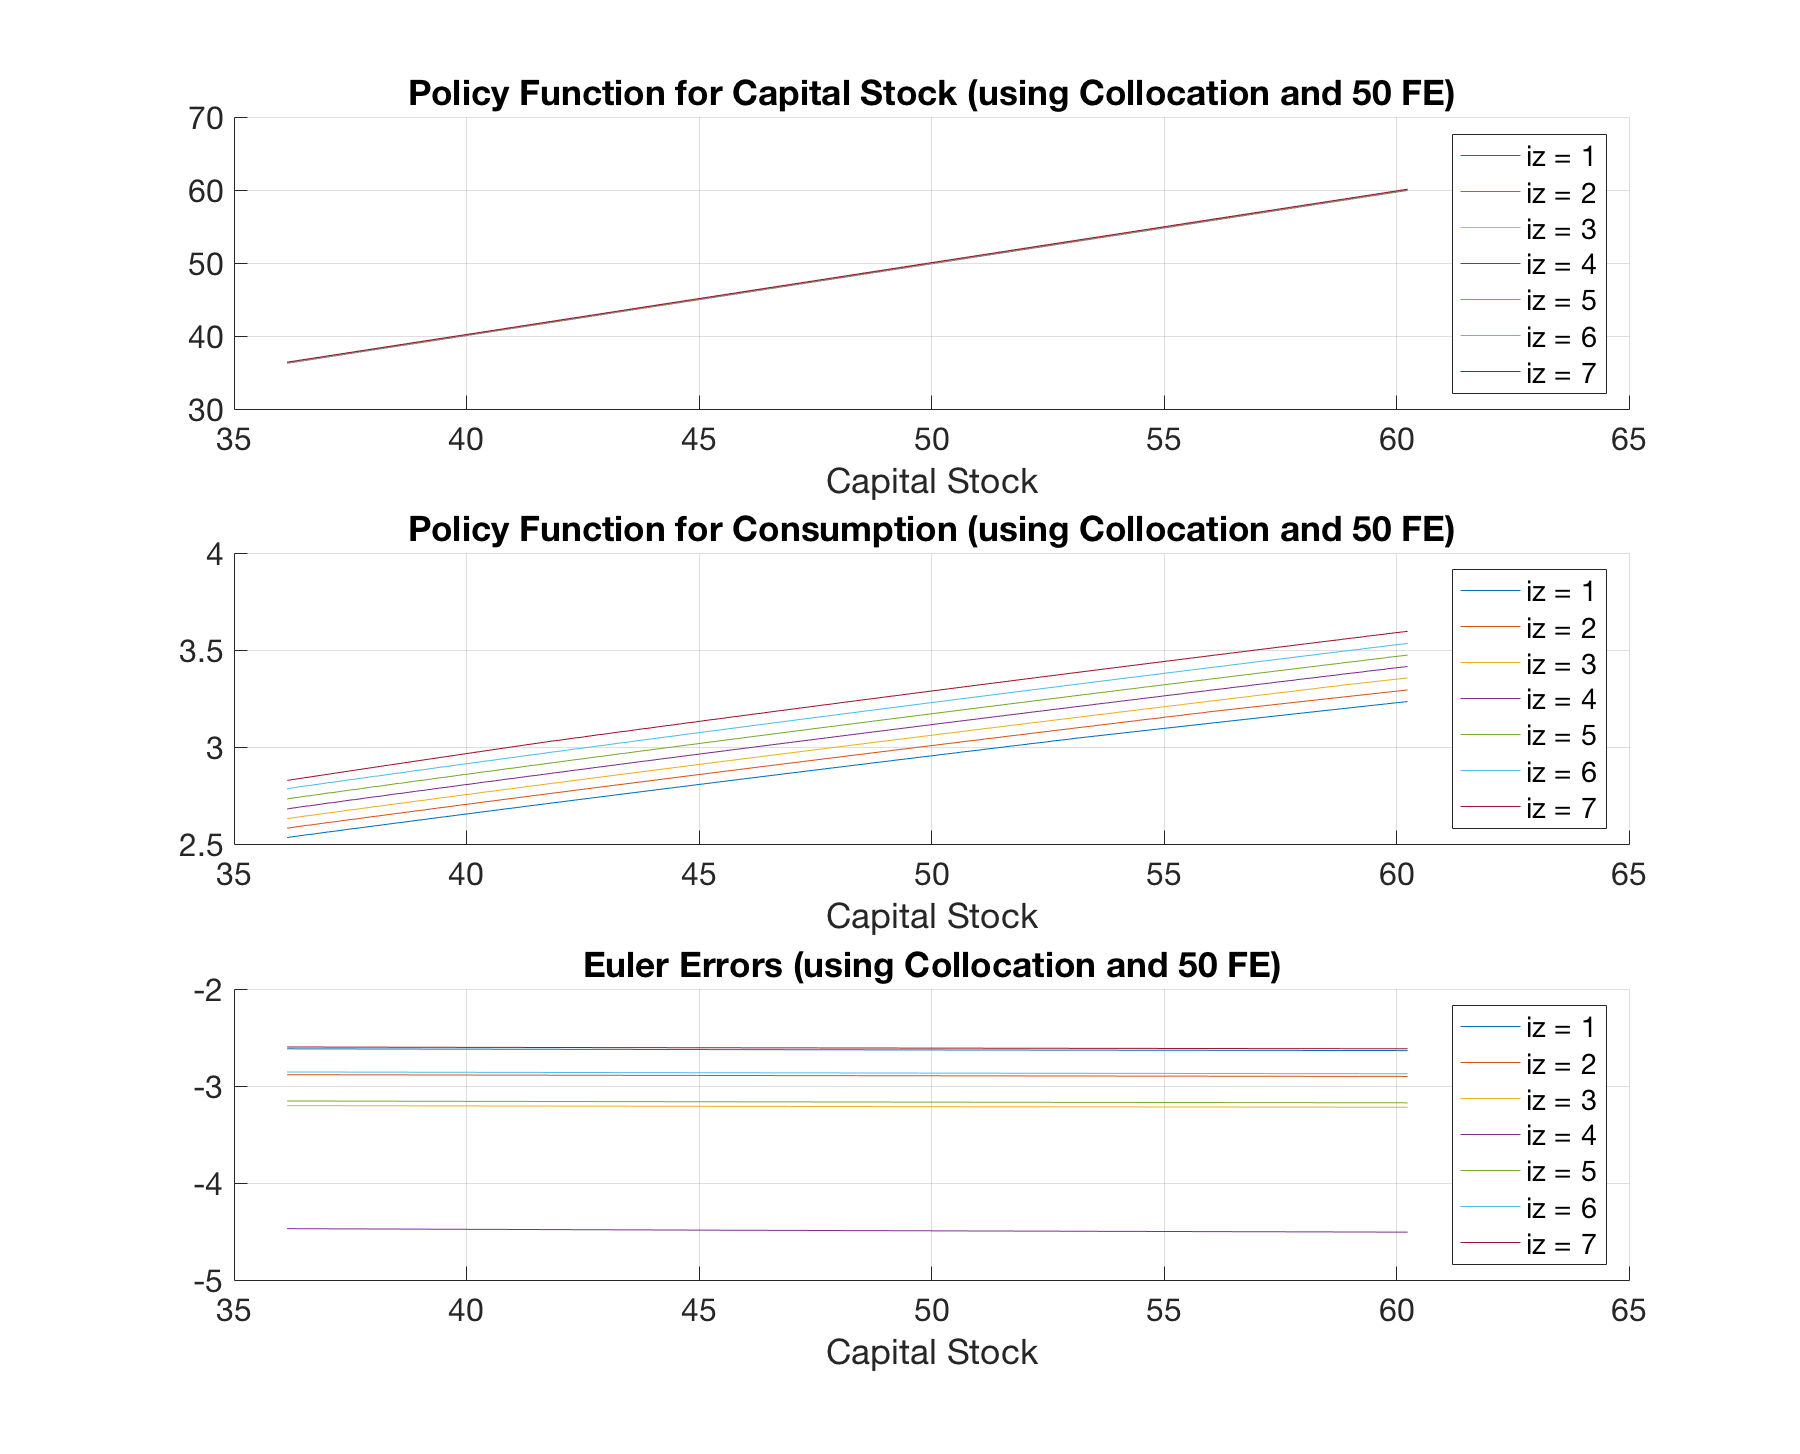
\includegraphics[scale = 0.25]{finel}
	\end{figure}
	
	Um outro gráfico interessante é o da diferença ponto a ponto em $(k, z)$ das duas soluções para a função política do consumo encontradas até agora, utilizando polinômios de Chebyshev e Elementos Finitos com Colocação:
	\begin{figure}[h!]
		\centering
		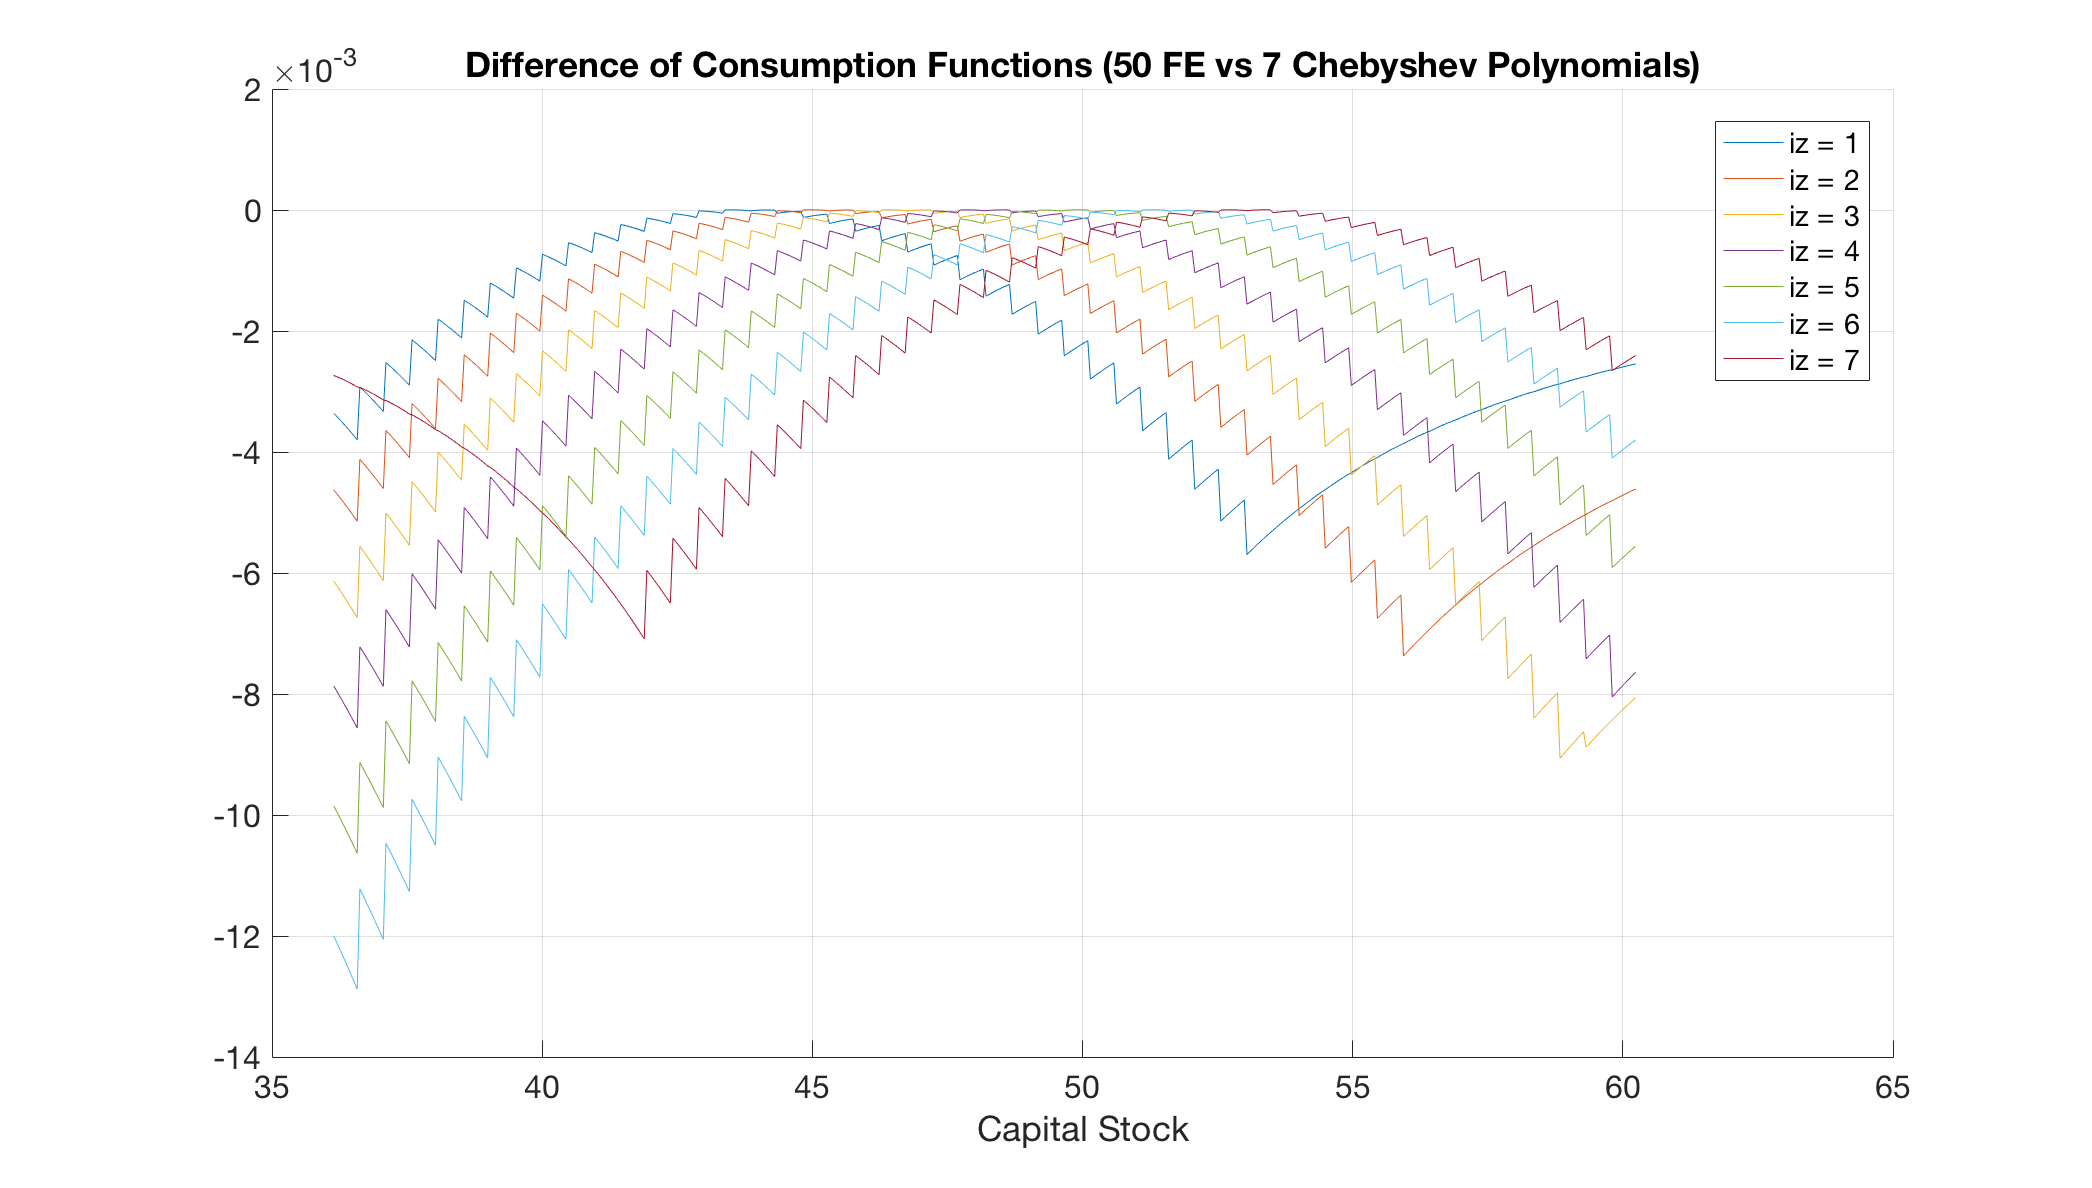
\includegraphics[scale = 0.2]{cheby_fe}
	\end{figure}
	
	A boa notícia é que a diferença (dos níveis) é bem pequena, da ordem de $10^{-2}$ no pior dos casos, quando o consumo varia aproximadamente entre $2.5$ e $4$ no estado estacionário. Curiosamente, esta diferença parece estar limitada superiormente por zero, isto é, parece ser o caso em que esta implementação de elementos finitos gera uma função política do consumo que está sempre acima daquela encontrada pelo método anterior. Contudo, é exatamente este o comportamento documentado nos slides ao comparar os polinômios de Chebyshev e o método de elementos finitos.
	
	Na segunda implementação utilizando elementos finitos, apliquei a técnica de Galerkin dos slides. A figura a seguir mostra que a solução encontrada é similar às outras, a menos de uma quina no caso de $iz = 4$. A diferença é que esta implementação mostrou-se MUITO mais demorada do que as outras: quase 10 \textit{minutos} se passaram até que a rotina \texttt{fsolve} conseguisse encontrar a solução.
	\begin{figure}[h!]
		\centering
		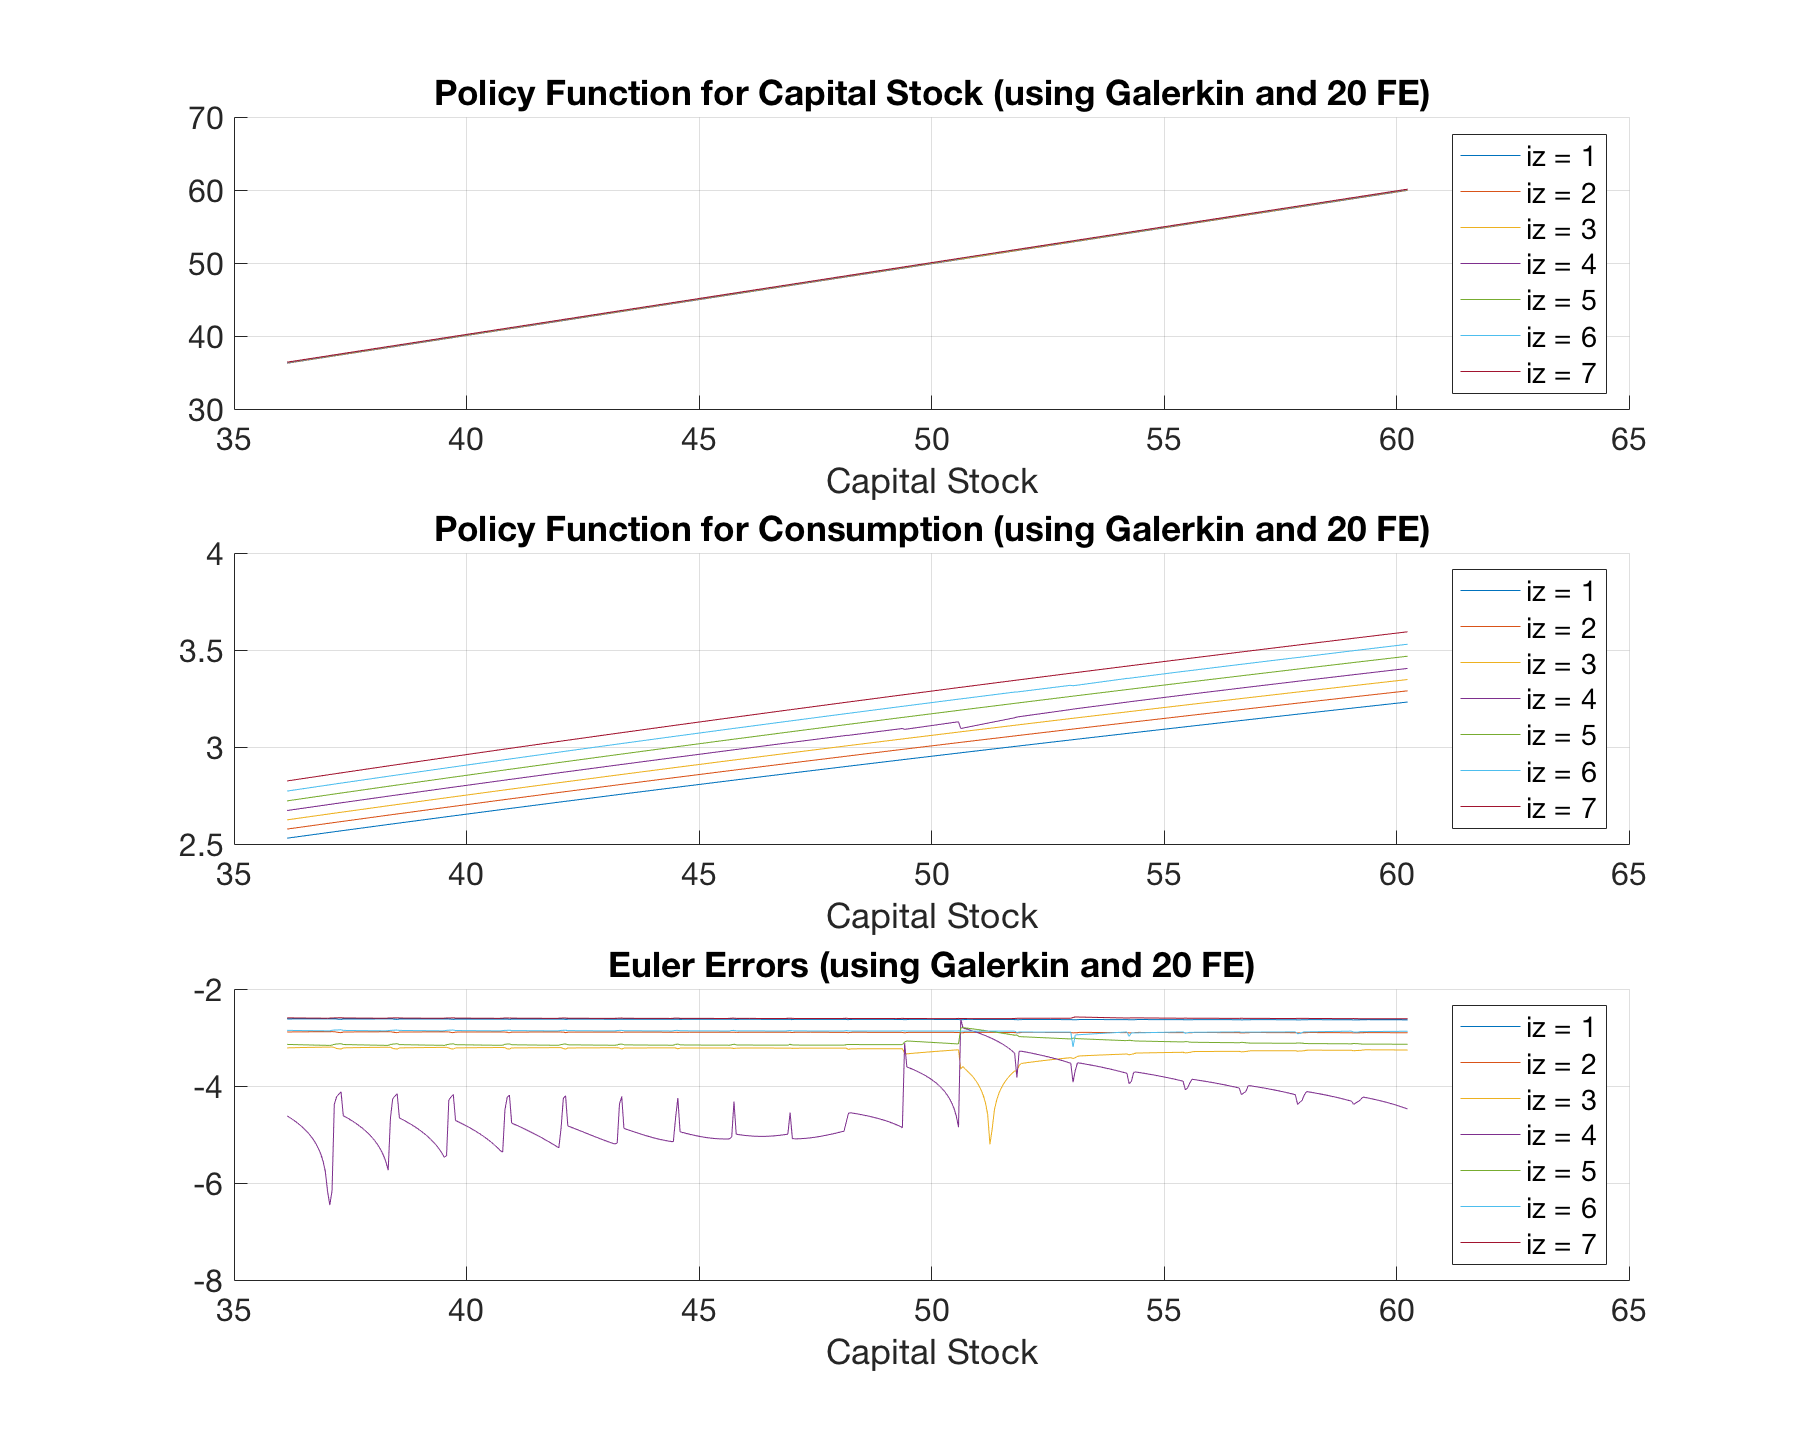
\includegraphics[scale = 0.25]{galerkin}
	\end{figure}
	
	Com poucos elementos finitos, a solução para a função política do capital continha muitas quinas. Tal qual o caso anterior, dentro de cada elemento a função política é uma função afim do capital. Portanto, foram computados 40 parâmetros, em vista dos 20 elementos finitos.
	
	Acredito que o motivo desta lentidão seja a necessidade de computar integrais numéricas. A função \texttt{risk\_function\_galerkin} utiliza as outras funções já desenvolvidas para a implementação com colocação e a rotina interna do MATLAB \texttt{integral} para computar 40 integrais numéricas em cada rodada de \texttt{fsolve}.
	
	De acordo com a documentação, este é o método default mais recomendado para a integração de funções unidimensionais no MATLAB, usando um tipo de quadratura dita ``globalmente adaptativa''. No entanto, o overhead criado por cada rodada de \texttt{fsolve} parece acumular-se rapidamente. No caso de usarmos, por exemplo, 5 elementos finitos a solução é encontrada em pouco menos de 30 segundos. Todavia, com várias quinas indesejáveis. Já com 10 elementos, o tempo de execução foi pouco mais de um minuto com menos quinas, mas ainda não tão bem comportada como a solução acima.
	
	Em conclusão, o método de Galerkin, ao requerer integração numérica, não se mostrou uma boa alternativa aos outros métodos já estudados para resolver este problema. A função política é suave o suficiente para que métodos de projeção global como o método dos Polinômios de Chebyshev sejam capazes de computá-la. O método de elementos finitos com colocação também se mostrou uma abordagem viável nesta questão.
\end{prob}
\end{document}
